\documentclass[12pt]{article}\usepackage[]{graphicx}\usepackage[]{color}
%% maxwidth is the original width if it is less than linewidth
%% otherwise use linewidth (to make sure the graphics do not exceed the margin)
\makeatletter
\def\maxwidth{ %
  \ifdim\Gin@nat@width>\linewidth
    \linewidth
  \else
    \Gin@nat@width
  \fi
}
\makeatother

\definecolor{fgcolor}{rgb}{0.345, 0.345, 0.345}
\newcommand{\hlnum}[1]{\textcolor[rgb]{0.686,0.059,0.569}{#1}}%
\newcommand{\hlstr}[1]{\textcolor[rgb]{0.192,0.494,0.8}{#1}}%
\newcommand{\hlcom}[1]{\textcolor[rgb]{0.678,0.584,0.686}{\textit{#1}}}%
\newcommand{\hlopt}[1]{\textcolor[rgb]{0,0,0}{#1}}%
\newcommand{\hlstd}[1]{\textcolor[rgb]{0.345,0.345,0.345}{#1}}%
\newcommand{\hlkwa}[1]{\textcolor[rgb]{0.161,0.373,0.58}{\textbf{#1}}}%
\newcommand{\hlkwb}[1]{\textcolor[rgb]{0.69,0.353,0.396}{#1}}%
\newcommand{\hlkwc}[1]{\textcolor[rgb]{0.333,0.667,0.333}{#1}}%
\newcommand{\hlkwd}[1]{\textcolor[rgb]{0.737,0.353,0.396}{\textbf{#1}}}%
\let\hlipl\hlkwb

\usepackage{framed}
\makeatletter
\newenvironment{kframe}{%
 \def\at@end@of@kframe{}%
 \ifinner\ifhmode%
  \def\at@end@of@kframe{\end{minipage}}%
  \begin{minipage}{\columnwidth}%
 \fi\fi%
 \def\FrameCommand##1{\hskip\@totalleftmargin \hskip-\fboxsep
 \colorbox{shadecolor}{##1}\hskip-\fboxsep
     % There is no \\@totalrightmargin, so:
     \hskip-\linewidth \hskip-\@totalleftmargin \hskip\columnwidth}%
 \MakeFramed {\advance\hsize-\width
   \@totalleftmargin\z@ \linewidth\hsize
   \@setminipage}}%
 {\par\unskip\endMakeFramed%
 \at@end@of@kframe}
\makeatother

\definecolor{shadecolor}{rgb}{.97, .97, .97}
\definecolor{messagecolor}{rgb}{0, 0, 0}
\definecolor{warningcolor}{rgb}{1, 0, 1}
\definecolor{errorcolor}{rgb}{1, 0, 0}
\newenvironment{knitrout}{}{} % an empty environment to be redefined in TeX

\usepackage{alltt}

\input{4mbapreamble}
\input{4mba3q}
\newcommand{\BeautifulSolution}{{\color{blue}\begin{proof}{\color{magenta}\dots beautifully clear and concise text to be inserted here\dots}\end{proof}}}

%%%%%%%%%%%%%%%%%%%%%%%%%%%%%%%%%%%
%% FANCY HEADER AND FOOTER STUFF %%
%%%%%%%%%%%%%%%%%%%%%%%%%%%%%%%%%%%
\usepackage{fancyhdr,lastpage}
\pagestyle{fancy}
\fancyhf{} % clear all header and footer parameters
%%%\lhead{Student Name: \theblank{4cm}}
%%%\chead{}
%%%\rhead{Student Number: \theblank{3cm}}
%%%\lfoot{\small\bfseries\ifnum\thepage<\pageref{LastPage}{CONTINUED\\on next page}\else{LAST PAGE}\fi}
\lfoot{}
\cfoot{{\small\bfseries Page \thepage\ of \pageref{LastPage}}}
\rfoot{}
\renewcommand\headrulewidth{0pt} % Removes funny header line
%%%%%%%%%%%%%%%%%%%%%%%%%%%%%%%%%%%
\IfFileExists{upquote.sty}{\usepackage{upquote}}{}
\begin{document}

\begin{center}
{\bf Mathematics 4MB3/6MB3 Mathematical Biology\\
\smallskip
2018 ASSIGNMENT 3}\\
\medskip
\underline{\emph{Group Name}}: \texttt{{\color{blue}The Infective Collective}}\\
\medskip
\underline{\emph{Group Members}}: {\color{blue}Aurora Basinski-Ferris, Michael Chong, Daniel Park, Daniel Presta}
\end{center}

\bigskip
\noindent
This assignment is {\bfseries\color{red} due in class} on \textcolor{red}{\bf Wednesday 28 February 2018 at 11:30am}.

\bigskip

\section*{Analysis of the standard SIR model with vital dynamics}

\SIRintro

\begin{enumerate}[(a)]

\item \SIRa
{\color{blue}\begin{proof}{\color{magenta}
First, we need to show that the population size ($N=S+I+R$) is constant. We note that the population size is constant if $dN/dt = dS/dt+dI/dt+dR/dt=0$, as this implies that the change in each compartment of the population results in overall no change. 
\begin{equation}
\begin{aligned}
& \frac{dS}{dt}+\frac{dI}{dt}+\frac{dR}{dt}\\
&=(\mu N-\frac{\beta}{N}SI-\mu S)+(\frac{\beta}{N}SI-\gamma I -\mu I)+(\gamma I-\mu R)\\
&= \mu (N-S-I-R)\\
&= \mu (N-N)\\
&= 0
\end{aligned}
\end{equation}

The biologically relevant region $\Delta$ is given by 
$$
\Delta = \{(S, I, R) : 0 \leq S,I,R \leq N, S+I+R = N\},
$$
since none of the compartments can have negative population nor exceed the total population. In order to show that $\Delta$ is a forward invariant set, we wish to show that if $(S_0, I_0, R_0) = (S(t_0), I(t_0), R(t_0)) \in \Delta$ at some time $t_0$, then $(S(t'), I(t'), R(t'))$ at $t' = t_0 + \varepsilon$. To show this we will prove that if any of the compartments are 0, then its derivative is non-negative, and if any of the compartments holds the entire population $N$, then its derivative is non-positive. This ensures that all compartments remain in $\Delta.$
\begin{itemize}
\item Suppose that $S=0$. Then $dS/dt = \mu N >0$.
\item Suppose that $S=N$. Then this forces $I = 0$ since $S+I+R = N$ and $S, I, R \geq 0$. Then $dS/dt = \mu N - \mu N = 0$.
\item Suppose that $I = 0$. Then $dI/dt = 0 - 0 - 0 = 0$. 
\item Suppose that $I = N$. Then this forces $S=0$ since $S+I+R = N$ and $S, I, R \geq 0$. Then $dI/dt = -N (\gamma + \mu) < 0$. 
\item Suppose that $R=0$. Then, $dR/dt=\gamma I$. As $I \in \Delta$, we have that $I \geq 0$. Thus, $dR/dt \geq 0$.
\item Suppose that $R=N$. Then this forces that $I=0$ since $S+I+R=N$ and $S,I, R \geq 0$. Thus, $dR/dt=-\mu N < 0$.
\end{itemize}
This then shows that none of the compartments can escape the biologically relevant region $\Delta$ provided that the initial condition is in $\Delta$.
}\end{proof}}

\item \SIRb
{\color{blue}\begin{proof}{\color{magenta}
To put the equations in the proportional form, we can consider the proportional quantities defined by $\tilde{S}=S/N$, $\tilde{I}=I/N$, and $\tilde{R}=R/N$. We then define a new set of differential equations based on these proportional quantities:
\begin{equation}
\begin{aligned}
\frac{d\tilde{S}}{dt} &= \mu - \frac{\beta}{N^2} SI - \frac{\mu S}{N} \\ 
&= \mu -\beta\tilde{S}\tilde{I}\\
\frac{d\tilde{I}}{dt}&=\frac{\beta}{N^2}SI-\frac{\gamma I}{N}-\frac{\mu I}{N} \\
&= \beta \tilde{S}\tilde{I} -\gamma \tilde{I} -\mu \tilde{I}\\
\frac{d\tilde{R}}{dt} &= \frac{\gamma I} {N} - \frac{\mu R }{N} \\
&= \gamma \tilde{I} - \mu \tilde{R} \\
\end{aligned}
\end{equation}
However this is equivalent to a scaled version of the original system:
\begin{equation}
\begin{aligned}
\frac{d\tilde S}{dt} = \frac{1}{N} \frac{dS}{dt} \\
\frac{d\tilde I}{dt} = \frac{1}{N} \frac{dI}{dt} \\
\frac{d\tilde R}{dt} = \frac{1}{N} \frac{dR}{dt}
\end{aligned}
\end{equation}
and so this system of population proportions is dynamically equivalent to the original system. 
}\end{proof}}

\item \SIRc
{\color{blue}\begin{proof}{\color{magenta}
In order to rewrite the equations using the dimensionless time coordinate $\tau=(\gamma + \mu)t$, we wish to write out the equations for $dS/d\tau$, $dI/d\tau$, and $dR/d\tau$. To do this, we note that $dS/d\tau = dS/dt * dt/d\tau$, $dI/d\tau = dI/dt * dt/d\tau$, and $dR/d\tau = dR/dt * dt/d\tau$. This yields the following equations: 

\begin{equation}
\begin{aligned}
\frac{dS}{d\tau} &= \frac{dS}{dt} \frac{dt}{d\tau} = \frac{dS}{dt} \frac{1}{\gamma + \mu} = \frac{\mu}{\gamma + \mu} - \frac{\beta}{\gamma + \mu} SI - \frac{\mu}{\gamma + \mu} S = \varepsilon - \R_0 SI - \varepsilon S\\
\frac{dI}{d\tau} &= \frac{dI}{dt} \frac{dt}{d\tau} = \frac{dI}{dt} \frac{1}{\gamma + \mu} = \frac{\beta}{\gamma + \mu} SI - \frac{\gamma}{\gamma + \mu} I - \frac{\mu}{\gamma + \mu}I = \R_0 SI - I\\
\frac{dR}{dt} &= \frac{dR}{d\tau} \frac{dt}{d\tau} = \frac{dR}{dt} \frac{1}{\gamma + \mu} = \frac{\gamma}{\gamma + \mu} I - \frac{\mu}{\gamma + \mu} R = (1-\varepsilon) I - \varepsilon R 
\end{aligned}
\end{equation}
These equations demonstrate that $\varepsilon$ is the dimensionless birth rate and $\R_0$ is the dimensionless transmission rate. Biologically, we note that $\gamma + \mu$ is the rate at which an individual leaves the infected class. Therefore, $\tau = t(\gamma + \mu)$ is a unitless scaling of time such that one unit is the mean infectious period (which is equal to $1/(\gamma + \mu)$). This implies that $\varepsilon = \mu/(\gamma + \mu)$ is the natural death rate per capita expressed as deaths per individual per mean infectious period. Finally, $\R_0$ is the mean number of secondary cases caused by a primary case in a fully susceptible population. We can see this because $\beta$ is the mean transmission rate and $1/(\gamma + \mu)$ is the mean infectious period. These parameters are good choices for non-dimensionalizing the equations because they have intuitive biological interpretations. This allows us to obtain external estimates for these parameters so that we do not have to estimate them from the data. For $\varepsilon$ for instance, if we can experimentally obtain the mean recovery period $(1/\gamma)$ and obtain a population-wise death rate from census data, we can estimate $\varepsilon$ independently of the data. 

Here we will estimate $\varepsilon$ for chicken pox. For simplicity, we can assume that mean life expectancy is 70 years. Then, $\mu=1/70 \, \textrm{year}^{-1}$.
Chicken-pox is known for full recovery to take about a week. 
Then, $\gamma = 1/7 \, \textrm{days}^{-1} = 365/7 \, \textrm{years}^{-1} \approx 52 \, \textrm{years}^{-1}$. 
Our estimate of $\varepsilon$ for chicken pox is
$$
\varepsilon = \frac{1/70}{1/70 + 52} \approx 0.00027
$$
For rubella, recovery period is approximately $1.5$ weeks. 
Then, $\gamma = 1/1.5 \, \textrm{weeks}^{-1} = 52/1.5 \, \textrm{weeks}^{-1} \approx 34.7 \, \textrm{years}^{-1}$.
Our estimate of $\varepsilon$ for rubella is
$$
\varepsilon = \frac{1/70}{1/70 + 34.7} \approx 0.00041
$$
}\end{proof}}

\item \SIRd
{\color{blue}\begin{proof}{\color{magenta}
In this question we take $R, S, I$ to be the proportional quantities; in other words, we take them to be what was previously referred to as $\tilde{R}$, $\tilde{S}$, and $\tilde{I}$.
The system is at equilibrium iff
$$
\frac{dS}{dt} = \frac{dI}{dt} = \frac{dR}{dt} = 0.
$$
Note that $dI/dt =0$ if and only if $I(\R_0 S - 1) = 0$ if and only if either $I = 0$ or $\R_0 S - 1 = 0$, (i.e. $S = 1/\R_0$). Note that if  $I = 0$ and $dS/dt = \varepsilon - \R_0 SI - \varepsilon S = 0$, then we must have $S = 1$, which gives the the $(\hat S, \hat I) = (0, 0)$ disease-free equilibrium (DFE).

Using the $dS/dt=0$ expression, we can solve for the corresponding $I$ value when $S=1/\R_0$. This yields $\varepsilon - \R_0I(1/\R_0)-\varepsilon S=0$. After rearranging this expression, we have that $I=\varepsilon (1-(1/\R_0))$. Thus, we note that we only have two equilibria, as $dI/dt=0$ is only satisfied when either $I=0$ or $\R_0S-1=0$, and we have just shown that each of these two conditions only happen at one distinct $(S,I)$ point.\\
The equilibrium expression $(\hat{S}, \hat{I}) = (1/\R_0, \varepsilon (1- 1/\R_0))$ is biologically relevant when $\R_0 \geq 1$. However, note that this equilibrium expression does not yield a second distinct equilibrium when $\R_0 =1$; in that case, the expression gives the disease free equilibrium. Thus, if $\R_0 = 1$, we have only the disease free equilibrium, while if  $R_0 >1$, we have a distinct endemic equilibrium. If $R_0 <1$, then we have that $\hat S > 1$ and $ \hat I < 0$, which is not biologically relevant. In summary, for all $R_0$, we have the existence of the disease free equilibrium. However, when $\R_0 >1$, we have the additional existence of an endemic equilibrium. 
}\end{proof}}

\item \SIRe
{\color{blue}\begin{proof}{\color{magenta}
To prove asymptotic stability for the endemic equilibrium, we examine the Jacobian given by the system $dS/dt=\varepsilon-\R_0SI-\varepsilon S$ and $dI/dt=\R_0SI-I$. We find that the Jacobian of this system is: 
\begin{equation}
\begin{bmatrix}
-\R_0I-\varepsilon & -\R_0S\\
\R_0 I & \R_0 S -1
\end{bmatrix}
\end{equation}
At the disease free equilibrium $(1, 0)$, this matrix is
\begin{equation}
\begin{bmatrix}
-\varepsilon 	& -\R_0\\
0				& \R_0  -1
\end{bmatrix}
\end{equation}
which has eigenvalues $\lambda_1 = - \varepsilon < 0 $ and $\lambda_2 = \R_0 - 1 < 0 $ when $\R_0 < 1$. 
Therefore, when $\R_0 < 1$, the disease-free equilibrium is locally asymptotically stable, since both eigenvalues are negative.

After plugging in the point for endemic equilibrium given by $(\hat{S},\hat{I})=(1/\R_0, \varepsilon(1-(1/\R_0))$, this matrix becomes:
\begin{equation}
\begin{bmatrix}
-\R_0\varepsilon & -1\\
\varepsilon(\R_0-1) & 0
\end{bmatrix}
\end{equation}
The eigenvalues of this of this matrix are:
$$
\lambda_1 = \frac{1}{2} \left( - \sqrt{\varepsilon} \sqrt{\varepsilon\R_0^2 - 4 \R_0 + 4} - \varepsilon \R_0\right) < 0
$$
and
$$
\lambda_2 = \frac{1}{2}\left(\sqrt{\varepsilon} \sqrt{\varepsilon\R_0^2 - 4 \R_0 + 4} - \varepsilon \R_0\right).
$$
Note that $\lambda_2 < 0$ if and only if 
\begin{equation}
\begin{aligned}
\varepsilon \R_0 > \sqrt\varepsilon \sqrt{\varepsilon\R_0^2 - 4 \R_0 + 4} \\
\varepsilon^2 \R_0^2 > \varepsilon (\varepsilon \R_0^2 - 4\R_0 + 4)\\
0 > -4 \R_0 + 4\\
-4 > -4 \R_0\\
1 < \R_0.
\end{aligned}
\end{equation}
which is when the endemic equilibrium is biologically relevant. \\
Thus, we have demonstrated that the endemic equilibrium is locally asymptotically stable when $R_0>1$ which is the biologically relevant region for the endemic equilibrium.

We note that we could have done an alternative proof for the disease free equilibrium stability using Lyapunov's Direct Method. We now show that second approach to the proof. Define $L(S, I, R) = I+R$, and let $(S_0, I_0, R_0) = (1- \delta_1, \delta_2, \delta_1 - \delta_2) \in \Delta$. We wish to show that $(S_\ast, I_\ast, R_\ast) = (1, 0, 0)$ is asymptotically stable using Lyapunov's Direct Method (Theorem 1 on Assignment 1).

We begin by checking the first condition in the theorem. We claim that the region  $\mathcal{O} \{(S,I,R) \in \Delta \ | \ I< \varepsilon(1-S)/(\R_0S)\} \subset \Delta$ . Thus, we wish to verify that $L(S,I,R)=0$ when $(S,I,R)=(1,0,0)$, and that $L(S,I,R)>0$ when $(S,I,R) \neq (1,0,0)$ and $(S,I,R) \in \mathcal{O}$. The first part of this condition is clearly true given that $L(S,I,R)=I+R$ and $I=0,\ R=0$ at $(S_\ast, I_\ast, R_\ast)$. We verify the second part of the first condition, as for $(S,I,R) \in \mathcal{O}$ we know that $I=0$ and $R=0$ only occur simultaneously if $S=1$. This is because for $(S,I,R) \in \mathcal{O} \subset \Delta$, we have that $S+I+R=1$. Therefore, one of $S$ or $I$ is non-zero. As $S,I \in \mathcal{O}$ have that $S,I \in [0,1]$, it must be that for $(S,I,R) \neq (S_\ast, I_\ast, R_\ast)$, $L(S,I,R)>0$. 

Next, we check the second condition in the theorem. Namely, we verify that $\dot{L}(S,I,R) <0$ for $\{ (S,I,R) \in \mathcal{O} \ | \ (S,I,R) \neq (1,0,0)\}$. We note that $\dot{L}(S,I,R) = dI/dt + dR/dt$. Thus, we wish to verify that $\R_0 SI - I + (1-\varepsilon) I - \varepsilon R <0$. Cancelling terms and using that $R=1-S-I$, we need to verify that $\R_0 SI - \varepsilon + \varepsilon S <0$. Now, if  $(S, I, R) \in \mathcal{O}$, then $I<\varepsilon(1-S)/\R_0S$, and 
$$
\dot L = \R_0 SI - \varepsilon + \varepsilon S < \R_0 S \frac{\varepsilon(1-S)}{\R_0 S}- \varepsilon + \varepsilon S = \varepsilon(1-S) - \varepsilon(1-S) = 0
$$
Thus, as the Lyapunov function $L(S,I,R)=I+R$ in the region $\mathcal{O}=\{(S,I,R) \in \Delta \ | \ I< \varepsilon(1-S)/\R_0S\}$ satisfies the conditions for asymptotic stability in Lyapunov's direct method, we have that the disease free equilibrium is locally asymptotically stable when $\R_0<1$.
}\end{proof}}

\item \SIRf
{\color{blue}\begin{proof}{\color{magenta}
Define $L(S, I, R) = I$ and let $(S_0, I_0, R_0) = (1- \delta_1, \delta_2, \delta_1 - \delta_2) \in \Delta$. We wish to show that $\mathcal{C} := \{(S, 0, R) | S+R = 1, S, R \geq 0\} \subset \mathcal{O} = \Delta$ is globally asymptotically stable using Lyapunov's Direct Method for Closed Invariant Sets (Theorem 2 on Assignment 1). 
First, $L(X) = I = 0$ for all $X = (S, 0, R) \in \mathcal{C}$, and if $X \in \Delta \setminus \mathcal{C}$, then $X = (S, \delta, R)$ for some $\delta >0$. We then have that $L(X) = I = \delta >0$ in $\Delta \setminus \mathcal{C}$. 
Then, consider $\dot{L}(X)$ where $X \in \Delta \setminus \mathcal{C}$.
\begin{equation}
\begin{aligned}
\dot L(X) = \frac{dL}{dt} = \frac{dI}{dt} = \R_0 S I - I.
\end{aligned}
\end{equation}
We can expand this to obtain 
\begin{equation}
\begin{aligned}
\dot L(X) &= \R_0 S I -  I \\
&= I \left( \R_0 S - 1 \right).
\end{aligned}
\end{equation}
However, if we assume that $\R_0 \leq 1$ and $X \not \in \mathcal{C}$, then $S < 1$ and therefore $\R_0 S <1$, i.e. $\R_0 S - 1 < 0$. It follows then that  
\begin{equation}
\begin{aligned}
\dot L(X) = I \left( \R_0 S - 1 \right) < 0
\end{aligned}
\end{equation}
as required. Since we have shown this for all $X \in \Delta \setminus \mathcal C$, by Lyapunov's Direct Method for Closed Invariant Sets, $\mathcal{C}$ is globally asymptotically stable.
}\end{proof}}

\item \SIRg
{\color{blue}\begin{proof}{\color{magenta}
Define $L(S, I) = (S+I) - (\Hat{S} \log{S} + \Hat{I} \log{I})$ and let $(S_0, I_0, R_0) = (1 - \delta_1, \delta_2, \delta_1 - \delta_2) \in \Delta$. We wish to show that the endemic equilibrium given by
$$(\Hat{S}, \Hat{I}) = \left(\frac{1}{\R_0}, \varepsilon \left(1 - \frac{1}{\R_0}\right)\right)$$
is globally asymptotically stable through the use of Lyapunov's Direct Method. We begin by defining the basin of attraction of the EE as an open, dense subset of $\Delta$. We define this subset as
\begin{equation*}
\begin{aligned}
\mathcal{P} = \left\{(S, I, R) \in \Delta \, | \, I > \frac{\varepsilon (1 - S)}{\R_0 S}\right\},
\end{aligned}
\end{equation*}
and note that $\mathcal{P}=\Delta \setminus \mathcal{O}$ with $\mathcal{O}$ given in part e). We then verify that $L(S, I)$ is positive definite on $\mathcal{P}$, such that $L(S, I) > L(\Hat{S}, \Hat{I})$ for all $(S, I) \in \mathcal{P} \setminus (\Hat{S}, \Hat{I})$. We observe the Hessian matrix of $L(S, I)$, given by
$$H (S, I) = \begin{bmatrix} -\frac{\Hat{S}}{S^2} & 0 \\ 0 & -\frac{\Hat{I}}{I^2} \end{bmatrix}.$$
Since the eigenvalues of $H$ are both negative, $L$ is concave up, or more precisely, $L$ is positive definite, with a global minimum on $\mathcal{P}$ at $(\Hat{S}, \Hat{I})$.
We then demonstrate that $\dot{L}$ is negative definite on $\mathcal{P}$. This proves that $L(S, I) > L(\Hat{S}, \Hat{I})$ for all $(S, I) \in \mathcal{P} \setminus (\Hat{S}, \Hat{I})$. We observe that
\begin{equation*}
\begin{aligned}
\dot{L} (S, I) &= \frac{\partial L}{\partial S} \cdot \frac{dS}{dt} + \frac{\partial L}{\partial I} \cdot \frac{dI}{dt} \\
&= \left(1 - \frac{\Hat{S}}{S}\right) (\varepsilon - \R_0 SI - \varepsilon S) + \left(1 - \frac{\Hat{I}}{I}\right) (\R_0 SI - I) \\
&= \left(1 - \frac{1}{\R_0 S}\right) (\varepsilon - \R_0 SI - \varepsilon S) \left(1 - \left(\varepsilon \left(1 - \frac{1}{\R_0}\right)\right) \frac{1}{I}\right) (\R_0 SI - I)
\end{aligned}
\end{equation*}
Simplifying, we obtain
$$\dot{L} (S, I) = \varepsilon \left(2 - \frac{1}{\R_0 S} - \R_0 S\right).$$
Examining the behaviour of $L(S, I)$ in some neighbourhood of $(\Hat{S}, \Hat{I}) \in \mathcal{P}$, we observe that when the equilibrium is approached from above, such that
$$\Hat{I} = \varepsilon\left(1 - \frac{1}{\R_0}\right) < \frac{\varepsilon(1 - S)}{\R_0 S} < I,$$
we have that $S < 1/\R_0$. This implies that
$$\dot{L} (S, I) < \varepsilon \left(2 - 1 - \R_0 \frac{1}{\R_0}\right) = \varepsilon(2 - 2) = 0.$$ 
Alternatively, when the equilibrium is approached from below, such that
$$\frac{\varepsilon(1 - S)}{\R_0 S} < \varepsilon \left(1 - \frac{1}{\R_0}\right) = \Hat{I} < I,$$
we have that $1/S < \R_0$. This also implies that
$$\dot{L} (S, I) < \varepsilon \left(2 - \frac{\R_0}{\R_0} - 1\right) = 0.$$
This shows that regardless of the approach to the EE, $\dot{L}(S, I)$ is negative definite on $\mathcal{P}$. Therefore, $L$ is a strict Lyapunov function for the EE on $\mathcal{P} \in \Delta$, and so by Lyapunov's Direct Method, we can say that the endemic equilibrium is globally asymptotically stable if $\R_0 > 1$.
}\end{proof}}

\item \SIRh
{\color{blue}\begin{proof}{\color{magenta}
($\Longrightarrow$) We begin our proof by assuming that the approach to the EE occurs via damped oscillations. We must show that under this assumption, $\varepsilon < \varepsilon^{\ast}$, where
$$\varepsilon^{\ast} = \frac{4(\R_0 - 1)}{\R_0^2}.$$
Once again, we simplify the model and ignore the $R$ component:
\begin{equation*}
\begin{aligned}
\frac{dS}{dt} &= \varepsilon - \R_0 SI - \varepsilon S \\
\frac{dI}{dt} &= \R_0 SI - I.
\end{aligned}
\end{equation*}
Through linearization, we obtain the following Jacobian matrix
\begin{equation}
\begin{bmatrix}
-\R_0\varepsilon & -1\\
\varepsilon(\R_0-1) & 0
\end{bmatrix}
\end{equation}
When evaluated at the endemic equilibrium, we observe that the Jacobian is given by
\begin{equation} \label{Jacobian}
J(\Hat{S}, \Hat{I}) = 
\begin{bmatrix}  
-\varepsilon \R_0 & -1 \\
\varepsilon (\R_0 - 1) & 0\\
\end{bmatrix}
\end{equation}
We know that if the equilibrium is approached via oscillatory dynamics, then the eigenvalues of the Jacobian matrix must be complex conjugates. 
Recall that the eigenvalues are given by
$$
\begin{aligned}
\lambda_1 &= \frac{1}{2} \left(- \sqrt{\varepsilon} \sqrt{\varepsilon\R_0^2 - 4 \R_0 + 4} - \varepsilon \R_0\right)\\
\lambda_2 &= \frac{1}{2}\left(\sqrt{\varepsilon} \sqrt{\varepsilon\R_0^2 - 4 \R_0 + 4} - \varepsilon \R_0\right).
\end{aligned}
$$
Since the eigenvalues of the Jacobian matrix must be complex conjugates, we must have the following:
\begin{equation*}
\varepsilon \R_0 ^2 - 4(\R_0 - 1) < 0 
\end{equation*}
Since $\varepsilon > 0$ in $\Delta$, we then have that
\begin{equation*}
\varepsilon < \frac{4(\R_0 - 1)}{\R_0 ^2},
\end{equation*}
as desired.


($\Longleftarrow$) The reverse proof is similar. Suppose we have that $\varepsilon < \varepsilon^{\ast}$, such that
\begin{equation} \label{cond}
\begin{aligned}
\varepsilon &< \frac{4(\R_0 - 1)}{\R_0 ^2}.
\end{aligned}
\end{equation}
Then, solving for the eigenvalues of $J(\Hat{S}, \Hat{I})$, we observe that
$$
\begin{aligned}
\lambda_1 &= \frac{1}{2} \left(- \sqrt{\varepsilon} \sqrt{\varepsilon\R_0^2 - 4 \R_0 + 4} - \varepsilon \R_0\right)\\
\lambda_2 &= \frac{1}{2}\left(\sqrt{\varepsilon} \sqrt{\varepsilon\R_0^2 - 4 \R_0 + 4} - \varepsilon \R_0\right).
\end{aligned}
$$
When 
$$
\varepsilon < \frac{4(\R_0 - 1)}{\R_0 ^2}
$$
we know that both eigenvalues are complex. Furthermore, their real parts ($-\varepsilon/2$) are negative.
Therefore, the endemic equilibrium is reached via damped oscillations. 

When pondering which familiar diseases could exhibit oscillatory dynamics near the endemic equilibrium, we must consider diseases with fluctuations in the growth and decay of the susceptible and infected populations. In other words, from our observations, we determined that infectious diseases with lower values of $\varepsilon$ will exhibit damped oscillatory behaviour near the EE, whereas diseases with higher values of $\varepsilon$ will converge monotonically towards the EE. From this assignment, we discovered that diseases with shorter mean infectious periods result in lower values for $\varepsilon$, and so we thus predict that childhood diseases such as chicken pox, the common cold, measles, and mumps will exhibit some level of damped oscillations near the equilibrium. Conversely, we would expect that a disease with a longer mean infectious period, such as herpes, will converge monotonically towards the endemic equilibrium, due to its significantly higher $\varepsilon$ value.
}\end{proof}}

\item \SIRi
{\color{blue}\begin{proof}{\color{magenta}
Recall that the Jacobian of the system (ignoring $R$) at the endemic equilibrium is given by
$$
\begin{bmatrix}
- \varepsilon \R_0 & - 1 \\
\varepsilon (\R_0 - 1) & 0
\end{bmatrix}
$$
where its characteristic equation is given by
$$
\lambda^2 + \varepsilon \R_0 \lambda + \varepsilon(\R_0 - 1) = 0
$$
Then, its eigenvalues are given by
$$
\lambda = \frac{-\varepsilon \R_0 \pm \sqrt{\varepsilon^2 \R_0^2 - 4 \varepsilon(\R_0 - 1)}}{2}.
$$
When
$$
\varepsilon < \frac{4 (\R_0 - 1)}{\R_0^2},
$$
the eigenvalues of the Jacobian matrix are given by
$$
\lambda = -\frac{\varepsilon \R_0}{2} \pm i \frac{\sqrt{4 \varepsilon (\R_0 - 1) - \varepsilon^2 \R_0^2}}{2}
$$
For convenience, denote
$$
\begin{aligned}
\eta &= \frac{\sqrt{4 \varepsilon (\R_0 - 1) - \varepsilon^2 \R_0^2}}{2}\\
\alpha &= -\frac{\varepsilon \R_0}{2}.
\end{aligned}
$$
Furthermore, denote corresponding eigenvectors by $\vec{v}_1 = \vec{a} + \vec{b} i$ and $\vec{v}_2 = \vec{a} - \vec{b} i$.
Consider the following linear system:
$$
\frac{d}{dt} \vec{x} = \begin{bmatrix}
- \varepsilon \R_0 & - 1 \\
\varepsilon (\R_0 - 1) & 0
\end{bmatrix} \vec{x},
$$
where
$$
\vec{x}(t) = \begin{bmatrix}
S(t)\\
I(t)
\end{bmatrix}
$$
Note that this model is not a biologically meaningful model but rather a qualitative model that we expect the SIR model to behave like near the endemic equilibrium.
Then, by the result derived from 3MB3 course, we find that the solution to this linear system is given by
$$
\vec{x}(t) = \left[c_1 \left(\cos (\eta t) \vec{a} - \sin (\eta t) \vec{b} \right) + c_2 \left(\sin (\eta t) \vec{a} + \cos (\eta t) \vec{b} \right)  \right] \exp(\alpha t),
$$
where $c_1, c_2$ are determined by the initial conditions.
Indeed, this shows that the oscillation is damped because $\alpha < 0$ (and the oscillatory dynamics are determined by the sine and cosine terms, and the exponential term determines the magnitude of the oscillations). Furthermore, period of damped oscillation is given by $2\pi/\eta$ which is equal to
$$
\frac{4\pi}{\sqrt{4 \varepsilon (\R_0 - 1) - \varepsilon^2 \R_0^2}}.
$$
Furthermore, $e$-folding time for decay of the amplitude of oscillation is given by
$$
-\frac{1}{\alpha} = \frac{2}{\varepsilon \R_0}
$$
Near the equilibrium, our original model should behave like the linear model.
Hence, we expect our original SIR model to have similar $e$-folding time as well as period as this system.
We want to confirm these facts numerically.

First, we need to load some packages:
\begin{knitrout}
\definecolor{shadecolor}{rgb}{0.969, 0.969, 0.969}\color{fgcolor}\begin{kframe}
\begin{alltt}
\hlkwd{library}\hlstd{(deSolve)}
\hlkwd{library}\hlstd{(dplyr)}
\end{alltt}
\end{kframe}
\end{knitrout}
Following the previous assignment, we start by writing the gradient function:
\begin{knitrout}
\definecolor{shadecolor}{rgb}{0.969, 0.969, 0.969}\color{fgcolor}\begin{kframe}
\begin{alltt}
\hlcom{## SIR gradient}
\hlstd{SIR.grad} \hlkwb{<-} \hlkwa{function}\hlstd{(}\hlkwc{t}\hlstd{,} \hlkwc{y}\hlstd{,} \hlkwc{param}\hlstd{) \{}
    \hlkwd{with}\hlstd{(}\hlkwd{as.list}\hlstd{(}\hlkwd{c}\hlstd{(param, y)), \{}
        \hlstd{dS} \hlkwb{<-} \hlstd{epsilon} \hlopt{-} \hlstd{R0} \hlopt{*} \hlstd{S} \hlopt{*} \hlstd{I} \hlopt{-} \hlstd{epsilon} \hlopt{*} \hlstd{S}
        \hlstd{dI} \hlkwb{<-} \hlstd{R0} \hlopt{*} \hlstd{S} \hlopt{*} \hlstd{I} \hlopt{-} \hlstd{I}
        \hlstd{dR} \hlkwb{<-} \hlstd{(}\hlnum{1}\hlopt{-}\hlstd{epsilon)} \hlopt{*} \hlstd{I} \hlopt{-} \hlstd{epsilon} \hlopt{*} \hlstd{R}

        \hlkwd{list}\hlstd{(}\hlkwd{c}\hlstd{(dS, dI, dR))}
    \hlstd{\})}
\hlstd{\}}
\end{alltt}
\end{kframe}
\end{knitrout}

Here, we will use $\R_0=1.5$ and $\varepsilon=1/20$ with initial conditions $S(0)=0.99, I(0)=0.01$.
First, we want to confirm the rate of exponential decay.
To illustrate that the rate of exponential decay matches our expected value, we plot 
$$
c_3 \exp(- \varepsilon \R_0 t/2) + \varepsilon(1- 1/\R_0)
$$
along with the prevalence curve where $c_3$ is found by trial and error to match the second peak in the figure below. 

\begin{knitrout}
\definecolor{shadecolor}{rgb}{0.969, 0.969, 0.969}\color{fgcolor}\begin{kframe}
\begin{alltt}
\hlcom{## set parameter}
\hlstd{par} \hlkwb{<-} \hlkwd{c}\hlstd{(}\hlkwc{R0}\hlstd{=}\hlnum{1.5}\hlstd{,} \hlkwc{epsilon}\hlstd{=}\hlnum{1}\hlopt{/}\hlnum{20}\hlstd{)}
\hlcom{## set initial value}
\hlstd{y} \hlkwb{<-} \hlkwd{c}\hlstd{(}\hlkwc{S}\hlstd{=}\hlnum{1}\hlopt{-}\hlnum{1e-2}\hlstd{,} \hlkwc{I}\hlstd{=}\hlnum{1e-2}\hlstd{,} \hlkwc{R}\hlstd{=}\hlnum{0}\hlstd{)}
\hlcom{## set time}
\hlstd{tvec} \hlkwb{<-} \hlkwd{seq}\hlstd{(}\hlnum{0}\hlstd{,} \hlnum{150}\hlstd{,} \hlkwc{by}\hlstd{=}\hlnum{0.1}\hlstd{)}

\hlcom{## run ode and put it into data frame}
\hlstd{df} \hlkwb{<-} \hlkwd{as.data.frame}\hlstd{(}\hlkwd{ode}\hlstd{(y, tvec, SIR.grad, par))}

\hlcom{## plot ode}
\hlkwd{plot}\hlstd{(tvec, df}\hlopt{$}\hlstd{I,} \hlkwc{type}\hlstd{=}\hlstr{"l"}\hlstd{,} \hlkwc{ylab}\hlstd{=}\hlstr{"proportion"}\hlstd{,} \hlkwc{xlab}\hlstd{=}\hlstr{"time"}\hlstd{,} \hlkwc{lwd}\hlstd{=}\hlnum{2}\hlstd{)}
\hlcom{## draw exponential}
\hlkwd{with}\hlstd{(}\hlkwd{as.list}\hlstd{(par),\{}
    \hlkwd{curve}\hlstd{(}\hlnum{0.05} \hlopt{*} \hlkwd{exp}\hlstd{(}\hlopt{-}\hlstd{epsilon} \hlopt{*} \hlstd{R0}\hlopt{*}\hlstd{x}\hlopt{/}\hlnum{2}\hlstd{)}\hlopt{+} \hlstd{epsilon} \hlopt{*} \hlstd{(}\hlnum{1}\hlopt{-}\hlnum{1}\hlopt{/}\hlstd{R0),} \hlkwc{add}\hlstd{=T,} \hlkwc{col}\hlstd{=}\hlnum{2}\hlstd{,} \hlkwc{lty}\hlstd{=}\hlnum{2}\hlstd{,} \hlkwc{lwd}\hlstd{=}\hlnum{2}\hlstd{)}
\hlstd{\})}
\hlcom{## add legend}
\hlkwd{legend}\hlstd{(}
    \hlstr{"topright"}\hlstd{,}
    \hlkwc{col}\hlstd{=}\hlkwd{c}\hlstd{(}\hlnum{1}\hlstd{,} \hlnum{2}\hlstd{),}
    \hlkwc{lty}\hlstd{=}\hlkwd{c}\hlstd{(}\hlnum{1}\hlstd{,} \hlnum{2}\hlstd{),}
    \hlkwc{lwd}\hlstd{=}\hlkwd{c}\hlstd{(}\hlnum{2}\hlstd{,}\hlnum{2}\hlstd{),}
    \hlkwc{legend}\hlstd{=}\hlkwd{c}\hlstd{(}\hlstr{"SIR prevalence"}\hlstd{,} \hlstr{"exponential"}\hlstd{)}
\hlstd{)}
\end{alltt}
\end{kframe}
\includegraphics[width=\maxwidth]{figure/exp_decay-1} 

\end{knitrout}

We find that the exponential curve matches subsequent peaks (after the second peak) of the prevalence curve. 
It does not match the first peak but we do not expect the SIR model to behave like its linearized model immediately.
Hence, the discrepancy between the exponential curve and the first peak prevalence does not necessarily imply that the rate of exponential decay is different from what we expected.
We expect the exponential curve to match the linear model much better.

To provide stronger evidence, we plot the linearized system along with the numerical solution to the ODE.
Note that the approximate solution converges to the $(0,0)$ equilibrium instead of the endemic equilibrum of the SIR model. 
Instead of plotting the approximate solution directly, we plot
$$
\vec{x} + \begin{bmatrix}
\frac{1}{\R_0}\\
\varepsilon(1- 1/\R_0)
\end{bmatrix}
$$
so that the approximate solution converges to the endemic equilibrium of the SIR model. 
We find $c_1, c_2$ numerically by minimizing the sum of squared difference between the initial condition of the ODE with the initial condition of the approximate solution (so that both curves start at the same place).
We compare prevalence as well as the phase portrait.
Once again, we plot the same exponential curve on top of prevalence curves.

\begin{knitrout}
\definecolor{shadecolor}{rgb}{0.969, 0.969, 0.969}\color{fgcolor}\begin{kframe}
\begin{alltt}
\hlcom{## approximate SIR model using linearization}
\hlstd{approxSIR} \hlkwb{<-} \hlkwa{function}\hlstd{(}\hlkwc{t}\hlstd{,} \hlkwc{y}\hlstd{,} \hlkwc{param}\hlstd{) \{}
    \hlkwd{with}\hlstd{(}\hlkwd{as.list}\hlstd{(param), \{}

        \hlcom{## endemic equilibrium}
        \hlstd{eq} \hlkwb{<-} \hlkwd{c}\hlstd{(}\hlnum{1}\hlopt{/}\hlstd{R0, epsilon} \hlopt{*} \hlstd{(}\hlnum{1}\hlopt{-}\hlnum{1}\hlopt{/}\hlstd{R0))}

        \hlcom{## solution}
        \hlstd{approxfun} \hlkwb{<-} \hlkwa{function}\hlstd{(}\hlkwc{t}\hlstd{,} \hlkwc{c1}\hlstd{,} \hlkwc{c2}\hlstd{) \{}
            \hlstd{(c1} \hlopt{*} \hlstd{(}\hlkwd{cos}\hlstd{(eta} \hlopt{*} \hlstd{t)} \hlopt{*} \hlstd{avec}
                   \hlopt{-} \hlkwd{sin}\hlstd{(eta} \hlopt{*} \hlstd{t)} \hlopt{*} \hlstd{bvec)} \hlopt{+}
                \hlstd{c2} \hlopt{*} \hlstd{(}\hlkwd{sin}\hlstd{(eta} \hlopt{*} \hlstd{t)} \hlopt{*} \hlstd{avec}
                      \hlopt{+} \hlkwd{cos}\hlstd{(eta} \hlopt{*} \hlstd{t)} \hlopt{*} \hlstd{bvec))} \hlopt{*} \hlkwd{exp}\hlstd{(alpha} \hlopt{*} \hlstd{t)} \hlopt{+} \hlstd{eq}
        \hlstd{\}}

        \hlcom{## jacobian}
        \hlstd{jac} \hlkwb{<-} \hlkwd{matrix}\hlstd{(}\hlkwd{c}\hlstd{(}\hlopt{-}\hlstd{epsilon}\hlopt{*}\hlstd{R0, epsilon}\hlopt{*}\hlstd{(R0}\hlopt{-}\hlnum{1}\hlstd{),} \hlopt{-}\hlnum{1}\hlstd{,} \hlnum{0}\hlstd{),} \hlnum{2}\hlstd{,} \hlnum{2}\hlstd{)}

        \hlcom{## find eigenvalues}
        \hlstd{ee} \hlkwb{<-} \hlkwd{eigen}\hlstd{(jac)}

        \hlstd{alpha} \hlkwb{<-} \hlkwd{Re}\hlstd{(ee}\hlopt{$}\hlstd{values[}\hlnum{1}\hlstd{])}
        \hlstd{eta} \hlkwb{<-} \hlkwd{Im}\hlstd{(ee}\hlopt{$}\hlstd{values[}\hlnum{1}\hlstd{])}

        \hlstd{avec} \hlkwb{<-} \hlkwd{Re}\hlstd{(ee}\hlopt{$}\hlstd{vectors[,}\hlnum{1}\hlstd{])}
        \hlstd{bvec} \hlkwb{<-} \hlkwd{Im}\hlstd{(ee}\hlopt{$}\hlstd{vectors[,}\hlnum{1}\hlstd{])}

        \hlcom{## find c1 and c2 that gives initial values}
        \hlstd{res} \hlkwb{<-} \hlkwd{optim}\hlstd{(}\hlkwc{par}\hlstd{=}\hlkwd{c}\hlstd{(}\hlnum{0}\hlstd{,} \hlnum{0}\hlstd{),} \hlkwc{fn}\hlstd{=}\hlkwa{function}\hlstd{(}\hlkwc{x}\hlstd{) \{}
            \hlkwd{sum}\hlstd{((y[}\hlkwd{c}\hlstd{(}\hlstr{"S"}\hlstd{,} \hlstr{"I"}\hlstd{)]}\hlopt{-}\hlkwd{approxfun}\hlstd{(}\hlkwd{min}\hlstd{(t),} \hlkwc{c1}\hlstd{=x[}\hlnum{1}\hlstd{],} \hlkwc{c2}\hlstd{=x[}\hlnum{2}\hlstd{]))}\hlopt{^}\hlnum{2}\hlstd{)}
        \hlstd{\})}

        \hlstd{pp} \hlkwb{<-} \hlstd{res}\hlopt{$}\hlstd{par}

        \hlcom{## compute linear solution}
        \hlstd{ss} \hlkwb{<-} \hlkwd{sapply}\hlstd{(t,} \hlkwa{function}\hlstd{(}\hlkwc{t}\hlstd{) \{}
            \hlkwd{c}\hlstd{(t,} \hlkwd{approxfun}\hlstd{(t,} \hlkwc{c1}\hlstd{=pp[}\hlnum{1}\hlstd{],} \hlkwc{c2}\hlstd{=pp[}\hlnum{2}\hlstd{]))}
        \hlstd{\},} \hlkwc{simplify}\hlstd{=}\hlnum{FALSE}\hlstd{)}

        \hlcom{## put it in a data frame}
        \hlstd{solution} \hlkwb{<-} \hlkwd{as.data.frame}\hlstd{(}\hlkwd{do.call}\hlstd{(}\hlstr{'rbind'}\hlstd{, ss))}

        \hlkwd{names}\hlstd{(solution)} \hlkwb{<-} \hlkwd{c}\hlstd{(}\hlstr{"time"}\hlstd{,} \hlstr{"S"}\hlstd{,} \hlstr{"I"}\hlstd{)}

        \hlstd{solution}
    \hlstd{\})}
\hlstd{\}}
\hlcom{## run function}
\hlstd{approxdf} \hlkwb{<-} \hlkwd{approxSIR}\hlstd{(tvec, y, par)}

\hlkwd{par}\hlstd{(}\hlkwc{mfrow}\hlstd{=}\hlkwd{c}\hlstd{(}\hlnum{1}\hlstd{,}\hlnum{2}\hlstd{))}
\hlcom{## plot}
\hlkwd{plot}\hlstd{(tvec, df}\hlopt{$}\hlstd{I,} \hlkwc{type}\hlstd{=}\hlstr{"l"}\hlstd{,} \hlkwc{lwd}\hlstd{=}\hlnum{2}\hlstd{,} \hlkwc{ylab}\hlstd{=}\hlstr{"proportion"}\hlstd{,} \hlkwc{xlab}\hlstd{=}\hlstr{"time"}\hlstd{)}
\hlkwd{lines}\hlstd{(tvec, approxdf}\hlopt{$}\hlstd{I,} \hlkwc{col}\hlstd{=}\hlnum{4}\hlstd{,} \hlkwc{lwd}\hlstd{=}\hlnum{2}\hlstd{)}
\hlkwd{with}\hlstd{(}\hlkwd{as.list}\hlstd{(par),\{}
    \hlkwd{curve}\hlstd{(}\hlnum{0.05} \hlopt{*} \hlkwd{exp}\hlstd{(}\hlopt{-}\hlstd{epsilon} \hlopt{*} \hlstd{R0}\hlopt{*}\hlstd{x}\hlopt{/}\hlnum{2}\hlstd{)}\hlopt{+}\hlstd{epsilon} \hlopt{*} \hlstd{(}\hlnum{1}\hlopt{-}\hlnum{1}\hlopt{/}\hlstd{R0),}
        \hlkwc{add}\hlstd{=}\hlnum{TRUE}\hlstd{,} \hlkwc{col}\hlstd{=}\hlnum{2}\hlstd{,} \hlkwc{lty}\hlstd{=}\hlnum{2}\hlstd{,} \hlkwc{lwd}\hlstd{=}\hlnum{2}\hlstd{)}
\hlstd{\})}
\hlkwd{legend}\hlstd{(}
    \hlstr{"topright"}\hlstd{,}
    \hlkwc{col}\hlstd{=}\hlkwd{c}\hlstd{(}\hlnum{1}\hlstd{,} \hlnum{2}\hlstd{,} \hlnum{4}\hlstd{),}
    \hlkwc{lty}\hlstd{=}\hlkwd{c}\hlstd{(}\hlnum{1}\hlstd{,} \hlnum{2}\hlstd{,} \hlnum{1}\hlstd{),}
    \hlkwc{lwd}\hlstd{=}\hlnum{2}\hlstd{,}
    \hlkwc{legend}\hlstd{=}\hlkwd{c}\hlstd{(}\hlstr{"SIR prevalence"}\hlstd{,} \hlstr{"exponential"}\hlstd{,} \hlstr{"linearization"}\hlstd{)}
\hlstd{)}
\hlkwd{title}\hlstd{(}\hlstr{"Comparison of prevalence curves"}\hlstd{)}

\hlkwd{plot}\hlstd{(df}\hlopt{$}\hlstd{S, df}\hlopt{$}\hlstd{I,} \hlkwc{type}\hlstd{=}\hlstr{"l"}\hlstd{,} \hlkwc{lwd}\hlstd{=}\hlnum{2}\hlstd{,} \hlkwc{xlab}\hlstd{=}\hlstr{"S"}\hlstd{,} \hlkwc{ylab}\hlstd{=}\hlstr{"I"}\hlstd{)}
\hlkwd{lines}\hlstd{(approxdf}\hlopt{$}\hlstd{S , approxdf}\hlopt{$}\hlstd{I,} \hlkwc{col}\hlstd{=}\hlnum{4}\hlstd{,} \hlkwc{lwd}\hlstd{=}\hlnum{2}\hlstd{)}
\hlkwd{title}\hlstd{(}\hlstr{"Comparison of phase portraits"}\hlstd{)}
\end{alltt}
\end{kframe}
\includegraphics[width=\maxwidth]{figure/approx-1} 

\end{knitrout}

We note that as time increases, the prevalence curve generated by the SIR model behaves like the linear model in both figures, confirming our prediction that the SIR model behaves like the linear model near the endemic equilibrium. Furthermore, the exponential curve we estimated previously agrees with the peaks of the linear model prevalence curve, again confirming our prediction about the $e$-folding time.
Since the curves (actual SIR and linear) overlap so well near the endemic equilibrium, we can say that their periods must be very similar as well. Hence, the period that we derived above is still valid.

}\end{proof}}

\item \SIRj
{\color{blue}\begin{proof}{\color{magenta}
When $\R_0 < 1$, the disease free equilibrium is globally asympotically stable and when $\R_0 > 1$, the endemic equilibrium is globally asymptotically stalbe. Hence, $\R_0 = 1$ is one bifurcation point.
Now, consider when $\R_0 > 1$.
Recall that damped oscillation occurs when
$$
\varepsilon < \frac{4(\R_0 - 1)}{\R_0^2}.
$$
Rearranging, we have
$$
\varepsilon \R_0^2 - 4 \R_0 + 4 < 0 \implies \frac{4 - \sqrt{16 - 16 \varepsilon}}{2 \varepsilon} < \R_0 < \frac{4 + \sqrt{16 - 16 \varepsilon}}{2 \varepsilon}.
$$
Hence, we find that
$$
\R_0 = \frac{4 - \sqrt{16 - 16 \varepsilon}}{2 \varepsilon}, \frac{4 - \sqrt{16 + 16 \varepsilon}}{2 \varepsilon}
$$
are two bifurcation points provided that
\begin{equation}\label{eq:epsilon}
\frac{4 - \sqrt{16 - 16 \varepsilon}}{2 \varepsilon} > 1.
\end{equation}

Recall again that the Jacobian of the system (ignoring $R$) at the endemic equilibrium is given by
$$
\begin{bmatrix}
- \varepsilon \R_0 & - 1 \\
\varepsilon (\R_0 - 1) & 0
\end{bmatrix}
$$
Its eigenvalues are given by
$$
\lambda = \frac{-\varepsilon \R_0 \pm \sqrt{\varepsilon^2 \R_0^2 - 4 \varepsilon(\R_0 - 1)}}{2}.
$$
So when 
$$
\R_0 < \frac{4 - \sqrt{16 - 16 \varepsilon}}{2 \varepsilon} \text{ or } \R_0 > \frac{4 + \sqrt{16 - 16 \varepsilon}}{2 \varepsilon},
$$
we no longer have complex eigenvalues and hence the oscillation disappears.

To show four bifurcations, we fix $\varepsilon^\ast = 0.4$. 
This is a good choice for epsilon because this value stisfies $\eqref{eq:epsilon}$:
$$
\frac{4 - \sqrt{16 - 16 \varepsilon^\ast}}{2 \varepsilon^\ast} = 1.127 > 1.
$$
Hence, four intervals that we are interested in are
$$
(0, 1), (1, 1.127), (1.127, 8.873), (8.873, \infty)
$$
We did not use $\epsilon = 8/9$ as suggested because $e$-folding time becomes much shorter than the period and oscillation becomes hard to observe. However, $\epsilon=8/9$ is a good choice as the bifurcation points are rational (1, 1.5, and 3).

\begin{knitrout}
\definecolor{shadecolor}{rgb}{0.969, 0.969, 0.969}\color{fgcolor}\begin{kframe}
\begin{alltt}
\hlcom{## set parameters for each}
\hlstd{par1} \hlkwb{<-} \hlstd{par2} \hlkwb{<-} \hlstd{par3} \hlkwb{<-} \hlstd{par4} \hlkwb{<-} \hlkwd{c}\hlstd{(}\hlkwc{R0} \hlstd{=} \hlnum{0.5}\hlstd{,} \hlkwc{epsilon}\hlstd{=}\hlnum{0.4}\hlstd{)}
\hlstd{par2[[}\hlstr{"R0"}\hlstd{]]} \hlkwb{<-} \hlnum{1.1}
\hlstd{par3[[}\hlstr{"R0"}\hlstd{]]} \hlkwb{<-} \hlnum{3}
\hlstd{par4[[}\hlstr{"R0"}\hlstd{]]} \hlkwb{<-} \hlnum{20}

\hlcom{## time}
\hlstd{tvec3} \hlkwb{<-} \hlkwd{seq}\hlstd{(}\hlnum{1}\hlstd{,} \hlnum{20}\hlstd{,} \hlkwc{by}\hlstd{=}\hlnum{0.01}\hlstd{)}
\hlstd{arrowt1} \hlkwb{<-} \hlnum{2.1}
\hlstd{arrowt2} \hlkwb{<-} \hlnum{2.3}

\hlcom{## function that draws phase plots}
\hlstd{phasefun} \hlkwb{<-} \hlkwa{function}\hlstd{(}\hlkwc{t}\hlstd{,} \hlkwc{y}\hlstd{,} \hlkwc{param}\hlstd{,} \hlkwc{...}\hlstd{) \{}
    \hlstd{df} \hlkwb{<-} \hlkwd{as.data.frame}\hlstd{(}\hlkwd{ode}\hlstd{(y, t, SIR.grad, param))}
    \hlkwd{lines}\hlstd{(df}\hlopt{$}\hlstd{S, df}\hlopt{$}\hlstd{I, ...)}
    \hlstd{a1} \hlkwb{<-} \hlstd{df[df}\hlopt{$}\hlstd{time}\hlopt{==}\hlstd{arrowt1,]}
    \hlstd{a2} \hlkwb{<-} \hlstd{df[df}\hlopt{$}\hlstd{time}\hlopt{==}\hlstd{arrowt2,]}
    \hlkwd{arrows}\hlstd{(}\hlkwc{x0}\hlstd{=a1}\hlopt{$}\hlstd{S,} \hlkwc{y0}\hlstd{=a1}\hlopt{$}\hlstd{I,} \hlkwc{x1}\hlstd{=a2}\hlopt{$}\hlstd{S,} \hlkwc{y1}\hlstd{=a2}\hlopt{$}\hlstd{I,} \hlkwc{length}\hlstd{=}\hlnum{0.05}\hlstd{)}
    \hlkwd{invisible}\hlstd{()}
\hlstd{\}}

\hlstd{ylist} \hlkwb{<-} \hlkwd{lapply}\hlstd{(}\hlkwd{seq}\hlstd{(}\hlnum{0.1}\hlstd{,} \hlnum{1}\hlstd{,} \hlkwc{by}\hlstd{=}\hlnum{0.1}\hlstd{),} \hlkwa{function}\hlstd{(}\hlkwc{i}\hlstd{)\{}
    \hlkwd{c}\hlstd{(}\hlkwc{S}\hlstd{=}\hlnum{1}\hlopt{-}\hlstd{i,} \hlkwc{I}\hlstd{=i,} \hlkwc{R}\hlstd{=}\hlnum{0}\hlstd{)}
\hlstd{\})}

\hlkwd{par}\hlstd{(}\hlkwc{mfrow}\hlstd{=}\hlkwd{c}\hlstd{(}\hlnum{2}\hlstd{,}\hlnum{2}\hlstd{))}
\hlkwd{plot}\hlstd{(}\hlnum{NA}\hlstd{,} \hlkwc{xlim}\hlstd{=}\hlkwd{c}\hlstd{(}\hlnum{0}\hlstd{,} \hlnum{1}\hlstd{),} \hlkwc{ylim}\hlstd{=}\hlkwd{c}\hlstd{(}\hlnum{0}\hlstd{,} \hlnum{1}\hlstd{),} \hlkwc{xlab}\hlstd{=}\hlstr{"S"}\hlstd{,} \hlkwc{ylab}\hlstd{=}\hlstr{"I"}\hlstd{)}
\hlkwd{abline}\hlstd{(}\hlkwc{a}\hlstd{=}\hlnum{1}\hlstd{,} \hlkwc{b}\hlstd{=}\hlopt{-}\hlnum{1}\hlstd{,} \hlkwc{lty}\hlstd{=}\hlnum{2}\hlstd{,} \hlkwc{col}\hlstd{=}\hlstr{"gray"}\hlstd{)}
\hlstd{L} \hlkwb{<-} \hlkwd{lapply}\hlstd{(ylist, phasefun,} \hlkwc{t}\hlstd{=tvec3,} \hlkwc{param}\hlstd{=par1)}
\hlstd{L} \hlkwb{<-} \hlkwd{lapply}\hlstd{(ylist,} \hlkwa{function}\hlstd{(}\hlkwc{x}\hlstd{)} \hlkwd{points}\hlstd{(}\hlkwc{x}\hlstd{=x[}\hlnum{1}\hlstd{],} \hlkwc{y}\hlstd{=x[}\hlnum{2}\hlstd{],} \hlkwc{pch}\hlstd{=}\hlnum{16}\hlstd{))}
\hlkwd{points}\hlstd{(}\hlnum{1}\hlstd{,} \hlnum{0}\hlstd{,} \hlkwc{pch}\hlstd{=}\hlnum{16}\hlstd{)}
\hlkwd{title}\hlstd{(}\hlstr{"Reproductive number: 0.5"}\hlstd{)}

\hlkwd{plot}\hlstd{(}\hlnum{NA}\hlstd{,} \hlkwc{xlim}\hlstd{=}\hlkwd{c}\hlstd{(}\hlnum{0}\hlstd{,} \hlnum{1}\hlstd{),} \hlkwc{ylim}\hlstd{=}\hlkwd{c}\hlstd{(}\hlnum{0}\hlstd{,} \hlnum{1}\hlstd{),} \hlkwc{xlab}\hlstd{=}\hlstr{"S"}\hlstd{,} \hlkwc{ylab}\hlstd{=}\hlstr{"I"}\hlstd{)}
\hlkwd{abline}\hlstd{(}\hlkwc{a}\hlstd{=}\hlnum{1}\hlstd{,} \hlkwc{b}\hlstd{=}\hlopt{-}\hlnum{1}\hlstd{,} \hlkwc{lty}\hlstd{=}\hlnum{2}\hlstd{,} \hlkwc{col}\hlstd{=}\hlstr{"gray"}\hlstd{)}
\hlstd{L} \hlkwb{<-} \hlkwd{lapply}\hlstd{(ylist, phasefun,} \hlkwc{t}\hlstd{=tvec3,} \hlkwc{param}\hlstd{=par2)}
\hlstd{L} \hlkwb{<-} \hlkwd{lapply}\hlstd{(ylist,} \hlkwa{function}\hlstd{(}\hlkwc{x}\hlstd{)} \hlkwd{points}\hlstd{(}\hlkwc{x}\hlstd{=x[}\hlnum{1}\hlstd{],} \hlkwc{y}\hlstd{=x[}\hlnum{2}\hlstd{],} \hlkwc{pch}\hlstd{=}\hlnum{16}\hlstd{))}
\hlkwd{points}\hlstd{(}\hlnum{1}\hlopt{/}\hlnum{1.1}\hlstd{,} \hlnum{0.4} \hlopt{*} \hlstd{(}\hlnum{1}\hlopt{-}\hlnum{1}\hlopt{/}\hlnum{1.1}\hlstd{),} \hlkwc{pch}\hlstd{=}\hlnum{16}\hlstd{)}
\hlkwd{title}\hlstd{(}\hlstr{"Reproductive number: 1.1"}\hlstd{)}

\hlkwd{plot}\hlstd{(}\hlnum{NA}\hlstd{,} \hlkwc{xlim}\hlstd{=}\hlkwd{c}\hlstd{(}\hlnum{0}\hlstd{,} \hlnum{1}\hlstd{),} \hlkwc{ylim}\hlstd{=}\hlkwd{c}\hlstd{(}\hlnum{0}\hlstd{,} \hlnum{1}\hlstd{),} \hlkwc{xlab}\hlstd{=}\hlstr{"S"}\hlstd{,} \hlkwc{ylab}\hlstd{=}\hlstr{"I"}\hlstd{)}
\hlkwd{abline}\hlstd{(}\hlkwc{a}\hlstd{=}\hlnum{1}\hlstd{,} \hlkwc{b}\hlstd{=}\hlopt{-}\hlnum{1}\hlstd{,} \hlkwc{lty}\hlstd{=}\hlnum{2}\hlstd{,} \hlkwc{col}\hlstd{=}\hlstr{"gray"}\hlstd{)}
\hlstd{L} \hlkwb{<-} \hlkwd{lapply}\hlstd{(ylist, phasefun,} \hlkwc{t}\hlstd{=tvec3,} \hlkwc{param}\hlstd{=par3)}
\hlstd{L} \hlkwb{<-} \hlkwd{lapply}\hlstd{(ylist,} \hlkwa{function}\hlstd{(}\hlkwc{x}\hlstd{)} \hlkwd{points}\hlstd{(}\hlkwc{x}\hlstd{=x[}\hlnum{1}\hlstd{],} \hlkwc{y}\hlstd{=x[}\hlnum{2}\hlstd{],} \hlkwc{pch}\hlstd{=}\hlnum{16}\hlstd{))}
\hlkwd{points}\hlstd{(}\hlnum{1}\hlopt{/}\hlnum{3}\hlstd{,} \hlnum{0.4} \hlopt{*} \hlstd{(}\hlnum{1}\hlopt{-}\hlnum{1}\hlopt{/}\hlnum{3}\hlstd{),} \hlkwc{pch}\hlstd{=}\hlnum{16}\hlstd{)}
\hlkwd{title}\hlstd{(}\hlstr{"Reproductive number: 3"}\hlstd{)}

\hlkwd{plot}\hlstd{(}\hlnum{NA}\hlstd{,} \hlkwc{xlim}\hlstd{=}\hlkwd{c}\hlstd{(}\hlnum{0}\hlstd{,} \hlnum{1}\hlstd{),} \hlkwc{ylim}\hlstd{=}\hlkwd{c}\hlstd{(}\hlnum{0}\hlstd{,} \hlnum{1}\hlstd{),} \hlkwc{xlab}\hlstd{=}\hlstr{"S"}\hlstd{,} \hlkwc{ylab}\hlstd{=}\hlstr{"I"}\hlstd{)}
\hlkwd{abline}\hlstd{(}\hlkwc{a}\hlstd{=}\hlnum{1}\hlstd{,} \hlkwc{b}\hlstd{=}\hlopt{-}\hlnum{1}\hlstd{,} \hlkwc{lty}\hlstd{=}\hlnum{2}\hlstd{,} \hlkwc{col}\hlstd{=}\hlstr{"gray"}\hlstd{)}
\hlstd{L} \hlkwb{<-} \hlkwd{lapply}\hlstd{(ylist, phasefun,} \hlkwc{t}\hlstd{=tvec3,} \hlkwc{param}\hlstd{=par4)}
\hlstd{L} \hlkwb{<-} \hlkwd{lapply}\hlstd{(ylist,} \hlkwa{function}\hlstd{(}\hlkwc{x}\hlstd{)} \hlkwd{points}\hlstd{(}\hlkwc{x}\hlstd{=x[}\hlnum{1}\hlstd{],} \hlkwc{y}\hlstd{=x[}\hlnum{2}\hlstd{],} \hlkwc{pch}\hlstd{=}\hlnum{16}\hlstd{))}
\hlkwd{points}\hlstd{(}\hlnum{1}\hlopt{/}\hlnum{20}\hlstd{,} \hlnum{0.4} \hlopt{*} \hlstd{(}\hlnum{1}\hlopt{-}\hlnum{1}\hlopt{/}\hlnum{20}\hlstd{),} \hlkwc{pch}\hlstd{=}\hlnum{16}\hlstd{)}
\hlkwd{title}\hlstd{(}\hlstr{"Reproductive number: 20"}\hlstd{)}
\end{alltt}
\end{kframe}
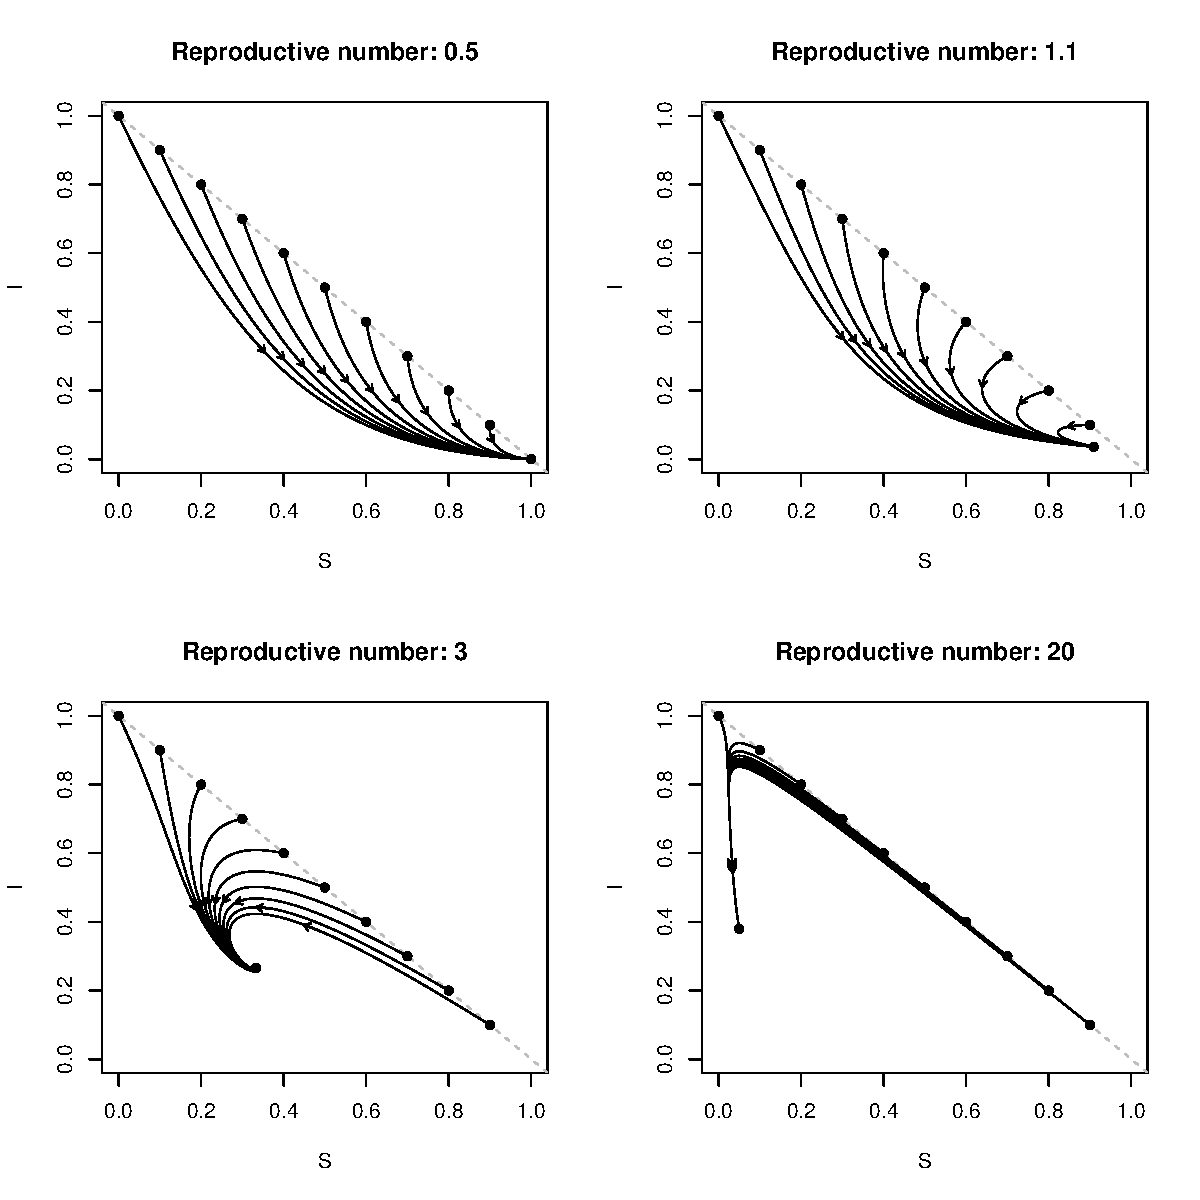
\includegraphics[width=\maxwidth]{figure/phase-1} 

\end{knitrout}


}\end{proof}}

\item \SIRk
{\color{blue}\begin{proof}{\color{magenta}
The model examined in this assignment doesn't describe the behaviour of most real diseases for small $\varepsilon$. The model predicts that for a small $\varepsilon$ value, there should be significant damped oscillations. This model falls short because while in many diseases we see recurrent behaviour that is explained with the oscillatory behaviour in the model, no disease have a clear and consistent decrease in prevalence at each oscillation. For example, if we look at a disease like measles, we note that $\varepsilon$ should be fairly low as the recovery period is short - this means that the probability of dying from natural causes before recovery is low. However, in measles, we see oscillatory behaviour but no clear decrease in prevalence at each oscillation (before vaccines were introduced). Specifically, if we look at the measles data in New York City (as presented in lecture), we found that a relatively high prevalence of the disease cycles either annually or biannually. 

To account for this behaviour and attempt to better fit the model to the data, we could introduce stochasticity. This stochastic behaviour would allow for the model to maintain the oscillatory behaviour while counteracting the dampening at each oscillation. However, as noted in part h, the model may be accurate at large $\varepsilon$, as at large $\varepsilon$, monotonic convergence is visible in many real diseases. For example, herpes has a large $\varepsilon$ value, as the recovery period is long. As would be expected by the model discussed in this assignment, herpes demonstrates monotonic convergence.

We might also consider that disease historically may have shown damped oscillatory behaviour, but has dampened to negligible amplitude since before data was collected. We would then only observe a near constant proportion of population infected, and it would be impossible to determine whether the dynamics of this disease agree with this model.
}\end{proof}}


\end{enumerate}

%\newpage
\bibliographystyle{vancouver}
\bibliography{DavidEarn,MyPubs}

\bigskip\vfill

\centerline{\bf--- END OF ASSIGNMENT ---}

\bigskip
Compile time for this document:
\today\ @ \thistime

\end{document}
